We would like to solve the thermal compliance problem
\begin{equation}\label{eq:thermal_compliance_problem}
    \begin{aligned}
        \min_{\rho} &\quad \int_\Omega f \cdot u \ \mathrm{d}x\\
        \text{s.t.} &\\
        &\quad\begin{cases}
            -\nabla \cdot (r(\tilde{\rho}) \nabla u) = f & \text{in } \Omega \text{ and BCs},\\
            - \epsilon^2 \Delta \tilde{\rho} + \tilde{\rho} = \rho & \text{in } \Omega \text{ and Neumann BCs},\\
            0 \leq \rho \leq 1 & \text{in } \Omega,\\
            \int_\Omega \rho\ \mathrm{d} x = \theta\cdot\text{vol}(\Omega),
        \end{cases}
    \end{aligned}
\end{equation}
over $u \in [H^1(\Omega)]^2$ and $\rho \in L^2(\Omega)$. Here, $r(\tilde{\rho}) = \rho_0 + \tilde{\rho}^3(1 - \rho_0)$
is the SIMP law,\\ $\epsilon$ is the design length scale, and $0 < \theta < 1$ is the volume fraction. Recall the
second constraint as the density filter for length parameter $\epsilon$.

\subsection{Method}

Breaking from the methodology in \texttt{toph.jl}, we will now use Keith and Surowiec's Entropic Mirror Descent algorithm (2023)
tailored to the constraint $\rho \in [0,1]$. Below, we will let $\sigma$ denote the sigmoid function, $\sigma^{-1}$
the inverse sigmoid function,
$\text{clip(y)} := \min(\text{max\_val}, \max(\text{min\_val}, y))$, and $\text{projit}(\psi)$ is a (compatible) projection
operator yet to be defined.

\begin{algorithm}
    \caption{Entropic Mirror Descent for PDE-constrained Topology Optimization}\label{alg:EMD}
    \begin{algorithmic}
    \Require $\mathcal{L}(u, \rho, \tilde{\rho}, w, \tilde{w})$ (the Lagrangian), $\alpha > 0$ (the step size)
    \Ensure $\rho = \argmin \int_\Omega f \cdot u \ \mathrm{d}x$
    \State $\psi \gets \sigma^{-1}(\theta)$ \Comment{So that $\int \sigma(\psi) = \theta \cdot \text{vol}(\Omega)$}
    \While{not converged}

        $\tilde{\rho} \gets$ solution to $\partial_{\tilde{w}} \mathcal{L} = 0$, \Comment{Filter solve}

        $u \gets$ state solution; solution to $\partial_{w} \mathcal{L} = 0$, \Comment{Primal problem}

        $\tilde{w} \gets$ filtered gradient; solution to $\partial_{\tilde{\rho}} \mathcal{L} = 0$,

        $G \gets M^{-1} \tilde{w}$; ie, is the solution to $(G,v) = (\tilde{w}, v)$ for all $v \in L^2$,

        $\psi \gets \text{clip}(\text{projit}(\psi - \alpha G))$. \Comment{Mirror descent update}

    \EndWhile
    \end{algorithmic}
\end{algorithm}
for the following discretization choices $u \in V \subset [H^1]^d$, $\psi \in L^2$ (with $\rho = \sigma(\psi)$),
$\tilde{\rho} \in H^1$, $w \in V$, $\tilde{w} \in H^1$, where
\begin{algorithm}
    \caption{projit($\psi$) Nonlinear Projection}
    \begin{algorithmic}
        \Require $\psi \in L^2(\Omega)$, $0 < \theta < 1$
        \Ensure $\int_{\Omega} \sigma(\psi + c)\ \mathrm{d}x = \theta \cdot \text{vol}(\Omega)$

        $c \gets$ Newton-Raphson result for $f(c) := \int_\Omega \sigma(\psi + c)\ \mathrm{d}x - \theta \text{vol}(\Omega)$
        
        $\psi \gets \psi + c$ \Comment{Performed in-place}
    \end{algorithmic}
\end{algorithm}
%%%%%%%%%%%%%%%%%%%%%%%%%%%%%%%%%%%%%%%%%%%%%%%%%%%%%%%%%%%%%%%%%%%%%%%%%%%%%%%%%%%%%%%%%%%%%%%%%%%%%
\subsection{Deriving the Lagrangian}

Following \cite{ghattas_willcox_2021}, we will be able to construct the required gradient using the Lagrangian; 
for this, we first require
the weak form of the forward problem. Note that neither of the conditions
on $\rho$ itself ([3] and [4] in the constraints to \autoref{eq:thermal_compliance_problem}) will be covered
here, as they are incorporated into and satisfied automatically as a result of the projection algorithm.

\subsubsection{Weak Form for Poisson}

For the PDE, we first multiply by a test
function $w$ and integrate over $\Omega$, yielding
\begin{equation}
    \int_\Omega - \nabla \cdot (r(\tilde{\rho}) \nabla u) \cdot w = \int_\Omega f \cdot w.
\end{equation}
Now, integrating by parts\footnote{Problem set 4; this is a result of the divergence theorem and the product rule for gradients.},
we expand the left hand side to reach
\begin{equation}\label{eq:Poisson_weak_form_1}
    -\int_{\partial \Omega} w(\nabla u) \cdot \mathbf{n} + \int_\Omega (r(\tilde{\rho})\nabla u) \cdot (\nabla w) = \int_\Omega f \cdot v.
\end{equation}

\subsubsection{Weak Form for Helmholtz type Diffusion}

We assume homogeneous Dirichlet boundary conditions, so it is safe to omit the boundary term as in \autoref{eq:Poisson_weak_form_1}.\footnote{
For a bit more detail, $u |_{\partial\Omega} = 0 \implies \nabla u \cdot \mathbf{n} |_{\partial\Omega} = 0$;
so, the integral on $\partial\Omega$ that appears is certainly $0$.} Since all integrals are over the same domain, we will
immediately write the inner products; multiplying by a test function $\tilde{w}$ and integrating, we begin with
\begin{equation}
    (-\epsilon^2 \Delta \tilde{\rho}, \tilde{w})_\Omega + (\tilde{\rho}, \tilde{w})_\Omega = (\rho, \tilde{w})_\Omega.
\end{equation}
Integrating by parts similarly, we reach
\begin{equation}
    (\epsilon^2 \nabla \tilde{\rho}, \nabla \tilde{w})_\Omega + (\tilde{\rho}, \tilde{w})_\Omega = (\rho, \tilde{w})_\Omega
\end{equation}
and are done.

\subsubsection{Constructing the Lagrangian from the Weak Forms}
Finally, noting that the objective can be written as $(f, u)$, we reach
\begin{multline}\label{eq:full_lagrangian}
    \mathcal{L}(u, \rho, \tilde{\rho}, w, \tilde{w}) = (f,u)_\Omega - (r(\tilde{\rho}) \nabla u, \nabla w)_\Omega + (\nabla u \cdot \mathbf{n}, w)_{\partial\Omega}\\
        + (f,w)_\Omega - (\epsilon^2 \nabla\tilde{\rho}, \nabla\tilde{w})_\Omega - (\tilde{\rho}, \tilde{w})_\Omega + (\rho, \tilde{w})_\Omega
\end{multline}

%%%%%%%%%%%%%%%%%%%%%%%%%%%%%%%%%%%%%%%%%%%%%%%%%%%%%%%%%%%%%%%%%%%%%%%%%%%%%%%%%%%%%%%%%%%%%%%%%%%%%
\subsection{The Gradient}

Following \cite{ghattas_willcox_2021} and to satisfy Keith and Surowiec's algorithm (2023), we work
towards the construction of the functional derivative $G$, for which we require the Gateaux derivatives
in each direction but $\rho$; these derivatives will recover several variational problems of interest.

First, we will recall the definition.

\begin{definition}[Gateaux Derivative]
    Let $X$ and $Y$ be Banach and $U \subseteq X$ be open. For $F: X \to Y$, the Gateaux differential
    of $F$ at $u \in U$ in the direction $\psi \in X$ is defined as
    \begin{equation}
        \frac{d}{dt} F(u + t\psi) \bigg|_{t=0}.
    \end{equation}
    $F$ is Gateaux differentiable at $u$ if the limit exists for all $\psi \in X$. Supposing $F$ is
    differentiable at $u$, the Gateaux derivative at $u$ will be denoted $\partial_u F$.
\end{definition}

We will assume basic linearity properties, which are fairly clear from the definition and essentially inherited from the linearity of the limit. The
following formulas will be useful. The first is rather intuitive.

\begin{lemma}[Gateaux derivative is zero against a ``constant functional'']\label{lem:zero_gateaux}
    Assuming that $v$ and $w$ are not functions of $u$, it holds that
    \begin{equation}
        \partial_u (v, w) = 0.
    \end{equation}
\end{lemma}
\begin{proof}
    Observe that
    \begin{equation*}
        \partial_u (v,w) = \frac{d}{dt} (v,w) \bigg|_{t=0} = 0 |_{t=0} = 0.
    \end{equation*}
\end{proof}

\begin{lemma}[Simple inner product formula]\label{lem:simple_gateaux}
    Assuming that $u, v \in L^2$,\footnote{Noticing our discretization choices from above, this will be sufficient for application.}
    It holds that
    \begin{equation}
        \partial_u (v, u) = (v, \psi).
    \end{equation}
    Moreover, by symmetry of the inner product, we have equivalently that
    \begin{equation}
        \partial_u (u, v) = (\psi, v).
    \end{equation}
\end{lemma}
\begin{proof}
    We will demonstrate the first and leave the second to symmetry.
    \begin{align*}
        \partial_u (v,u) &= \frac{d}{dt} (v, u + t\psi) \bigg|_{t=0} \\
            &= \frac{d}{dt} \int_\Omega v \cdot (u + t \psi),
    \end{align*}
    but this is
    \begin{equation*}
        \lim_{t \to 0} \frac{\int_\Omega v \cdot (u + t \psi) - \int_\Omega v \cdot u}{t} = \lim_{t \to 0}\frac{t \int_\Omega v \cdot \psi }{t} = \int_\Omega v \cdot \psi,
    \end{equation*}
    as desired.
\end{proof}

\begin{lemma}[Poisson weak form LHS formula]\label{lem:nabla_gateaux}
    Under the same conditions, it holds that
    \begin{equation}
        \partial_u (\nabla v, \nabla u) = (\nabla v, \nabla\psi)
    \end{equation}
    Moreover,
    \begin{equation}
        \partial_u (\nabla u, \nabla v) = (\nabla u, \nabla\psi)
    \end{equation}
    holds also by symmetry.
\end{lemma}
\begin{proof}
    We will demonstrate the first and leave the second to symmetry.
    \begin{align*}
        \partial_u (\nabla v,\nabla u) &= \frac{d}{dt} (\nabla v, \nabla( u + t\psi)) \bigg|_{t=0} \\
            &= \frac{d}{dt} (\nabla v, t \nabla \psi)\bigg|_{t=0} \\
            &= (\nabla v, \nabla \psi),
    \end{align*}
    where the second equality holds by \autoref{lem:zero_gateaux} and the third by bilinearity 
    and evaluation of the derivative and its restriction (notice $t$ disappears in the derivative).
\end{proof}

\subsubsection{Filter Equation}

Taking the derivative $\partial_{\tilde{w}} \mathcal{L}$, we will obtain the filter equation. Skipping the
application of \autoref{lem:zero_gateaux}, we have
\begin{align*}
    \partial_{\tilde{w}} \mathcal{L} &= \partial_{\tilde{w}} \left[ -(\epsilon^2 \nabla \tilde{\rho}, \nabla \tilde{w}) - (\tilde{\rho}, \tilde{w}) + (\rho, \tilde{w})\right] \\
        &= -(\epsilon^2 \nabla \tilde{\rho}, \nabla v) - (\tilde{\rho}, v) + (\rho, v),
\end{align*}
by \autoref{lem:nabla_gateaux} and \autoref{lem:simple_gateaux}.
Setting this equal to zero and moving terms around, solving the filter equation is to find $\tilde{\rho}$ such that
\begin{equation*}
    (\epsilon^2 \nabla \tilde{\rho}, \nabla v) + (\tilde{\rho}, v) = (\rho, v) \qquad \forall v \in H^1.
\end{equation*}

\subsubsection{Primal Problem}

Taking the derivative $\partial_{w} \mathcal{L}$, we will obtain the primal problem (state evaluation). Again skipping the application
of \autoref{lem:zero_gateaux}, we have
\begin{align*}
    \partial_{w} \mathcal{L} &= \partial_{w} \left[ -(r(\tilde{\rho}) \nabla u, \nabla w) + (\nabla u \cdot \mathbf{n}, w) + (f, w) \right]\\
        &= -(r(\tilde{\rho}) \nabla u, \nabla v) + (\nabla u \cdot \mathbf{n}, v) + (f,v).
\end{align*}
We would now like to find $u$ such that
\begin{equation*}
    (r(\tilde{\rho}) \nabla u, \nabla v) - (\nabla u \cdot \mathbf{n}, v) = (f,v) \qquad \forall v \in V.
\end{equation*}

\subsubsection{Dual Problem}

Taking the derivative $\partial_u \mathcal{L}$ yields the dual problem.
\begin{align*}
    \partial_{u} \mathcal{L} &= \partial_{u} \left[ (f,u) -(r(\tilde{\rho}) \nabla u, \nabla w) + (\nabla u \cdot \mathbf{n}, w) \right]\\
        &= -(r(\tilde{\rho}) \nabla v, \nabla w) + \partial_u(\nabla u \cdot \mathbf{n}, w)_{\partial\Omega} + (f,u),
\end{align*}
for all of which we have formulas excepting the boundary term. For this derivative,
\begin{align*}
    \partial_u (\nabla u \cdot \mathbf{n}, w) &= \frac{d}{dt} (\nabla(u + tv)\cdot\mathbf{n}, w) \bigg|_{t=0}\\
        &= \frac{d}{dt} t(\nabla v \cdot \mathbf{n}, w) \bigg|_{t=0}\\
        &= (\nabla v \cdot \mathbf{n}, w)
\end{align*}
by the linearity of $\nabla$ and properties of the dot product. So,
\begin{equation*}
    \partial_u \mathcal{L} = -(r(\tilde{\rho}) \nabla v, \nabla w) + (\nabla v \cdot \mathbf{n}, w) + (f,v).
\end{equation*}
Again setting this equal to zero, we would now like to find $w$ such that
\begin{equation*}
    (r(\tilde{\rho}) \nabla v, \nabla w) - (\nabla v \cdot \mathbf{n}, w) = (f,v) \qquad \forall v \in V.
\end{equation*}
By appealing again to symmetry, we see that this is identical to the primal problem.

\subsubsection{Filtered Gradient}

We require finally $\partial_{\tilde{\rho}} \mathcal{L}$.
\begin{align*}
    \partial_{\tilde{\rho}} \mathcal{L} &= \partial_{\tilde{\rho}} [-(r(\tilde{\rho}) \nabla u, \nabla w) - (\epsilon^2 \nabla \tilde{\rho}, \nabla \tilde{w}) - (\tilde{\rho}, \tilde{w})] \\
        &= - (\epsilon^2 \nabla v, \nabla\tilde{w}) - (v, \tilde{w}) - \partial_{\tilde{\rho}} (r(\tilde{\rho}) \nabla u, \nabla w)\\
        &= - (\epsilon^2 \nabla \tilde{w}, \nabla v) - (\tilde{w}, v) - \partial_{\tilde{\rho}} (r(\tilde{\rho}) \nabla u, \nabla w).
\end{align*}
For the derivative of the third term, for convenience, the SIMP law $r(\tilde{\rho})$ is provided again for convenience. $\rho_0$ denotes
the minimum value $\rho$ may take on and is used for numerical reasons; typically, this will be set a relatively very small value, like \texttt{1e-6}.
\begin{equation*}
    r(\tilde{\rho}) := \rho_0 + \tilde{\rho}^3 (1 - \rho_0)
\end{equation*}
So,
\begin{equation*}
    r'(\tilde{\rho}) = 3 \cdot \tilde{\rho}^2 (1 - \rho_0).
\end{equation*}
Now, with the differential interpass being justified under the functions' regularity and the dominated convergence theorem,
\begin{align*}
    \partial_{\tilde{\rho}} (r(\tilde{\rho}) \nabla u, \nabla w) &= \frac{d}{dt} (r(\tilde{\rho} + tv) \nabla u, \nabla w) \bigg|_{t=0}\\
        &= (r'(\tilde{\rho} + tv)v \nabla u, \nabla w) \bigg|_{t=0}\\
        &= (r'(\tilde{\rho})\nabla w \nabla u, v)\\
        &= (r'(\tilde{\rho}) |\nabla u|^2, v),
\end{align*}
by the equivalence of the primal and dual problems (ergo their solutions; it is from this that we deduce the final equivalence). Setting
the derivative equal to zero, we would like to find $\tilde{\rho}$ satisfying
\begin{equation*}
    (\epsilon^2 \nabla \tilde{w}, \nabla v) + (\tilde{w}, v) = (-r'(\tilde{\rho}) |\nabla u|^2, v), \qquad \forall v \in H^1.
\end{equation*}


%%%%%%%%%%%%%%%%%%%%%%%%%%%%%%%%%%%%%%%%%%%%%%%%%%%%%%%%%%%%%%%%%%%%%%%%%%%%%%%%%%%%%%%%%%%%%%%%%%%%%
\subsection{Examples}

We will now simulate a few problems over varying domains subject to varying boundary conditions. What remains is to describe the design domains $\Omega$ and
apply boundary conditions as appropriate.

\subsubsection{Unit Square with Single Sink}\label{sec:thermal_compliance_classic_unit_square}

We will first implement the problem solved in \texttt{toph.jl},
that is, solve \autoref{eq:thermal_compliance_problem} over the unit square under uniform, constant heating.
Heat is allowed to escape through the top third (marked blue; corresponding to $0$ Dirichlet boundary conditions),
and elsewhere there is no flow (corresponding to $0$ Neumann boundary conditions).
The following simulation was run with step-size $\alpha = 0.1$ and mass fraction $\theta = 0.4$.
\begin{figure}[ht]
    \centering
    \caption[b]{$\Omega$ for the first heat conduction problem.}
    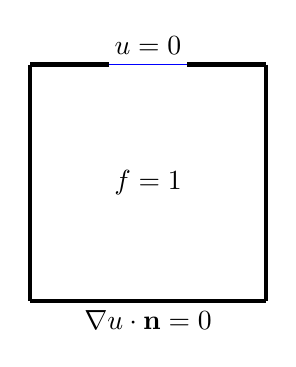
\begin{tikzpicture}
        \draw [ultra thick] (0,0) -- (0,3);
        \draw [ultra thick] (0,0) -- (3,0);
        \draw [ultra thick] (3,3) -- (2,3);
        \draw [blue] (2,3) -- (1,3);
        \draw [ultra thick] (1,3) -- (0,3);
        \draw [ultra thick] (3,3) -- (3,0);

        \node at (1.5, 3) [anchor = south] {$u = 0$};
        \node at (1.5, 1.5) {$f = 1$};
        \node at (1.5, 0) [anchor = north] {$\nabla u \cdot \mathbf{n} = 0$};
    \end{tikzpicture}
\end{figure}
Briefly on the physicality of the solution, first, note that the problem can be interpreted as the construction
of a heat sink within $\Omega$ for which we specify heating loads and where the heat is to dissipate out to, in
this case the load being uniform and constant over $\Omega$ (ie, the heating that the heat sink is subjected to
is uniform throughout the domain) with the heat being able to dissipate out one end.

We see, generally, the sort of surface area maximization that intuition would serve with the tree-like branching,
just as we observe the presence of triangles in solutions to the \texttt{top88.jl} structural compliance problems.


\subsubsection{Unit Square with Two Sinks}

Here, we allow for heat to escape also through a second port; due to the homogeneous boundary conditions, we end up with
an identical problem excepting the boundary condition specification (ie, there are still no boundary terms). This amounts
to a minor change in the boundary element labeling in the implementation (ie, that the lower third must now also be
identified with the same attribute as the top third).

\begin{figure}[H]
    \centering
    \caption[b]{$\Omega$ with two sinks.}
    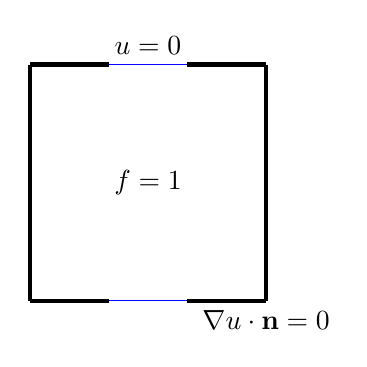
\begin{tikzpicture}
        \draw [ultra thick] (0,0) -- (0,3);

        \draw [ultra thick] (0,0) -- (1,0);
        \draw [blue] (1,0) -- (2,0);
        \draw [ultra thick] (2,0) -- (3,0);

        \draw [ultra thick] (3,3) -- (2,3);
        \draw [blue] (2,3) -- (1,3);
        \draw [ultra thick] (1,3) -- (0,3);

        \draw [ultra thick] (3,3) -- (3,0);

        \node at (1.5, 3) [anchor = south] {$u = 0$};
        \node at (1.5, 1.5) {$f = 1$};
        \node at (3, 0) [anchor = north] {$\nabla u \cdot \mathbf{n} = 0$};
    \end{tikzpicture}
\end{figure}


\vfill\pagebreak

\begin{figure}[H]
    \centering
    \caption{Unit Square with Single Sink: Filtered Distribution}
    \begin{subfigure}{.4\textwidth}
        
\includegraphics[width=\textwidth]{imgs/UnitSquare_1/first.png}
        \caption{$t = 1$}
    \end{subfigure}
    \begin{subfigure}{.4\textwidth}
        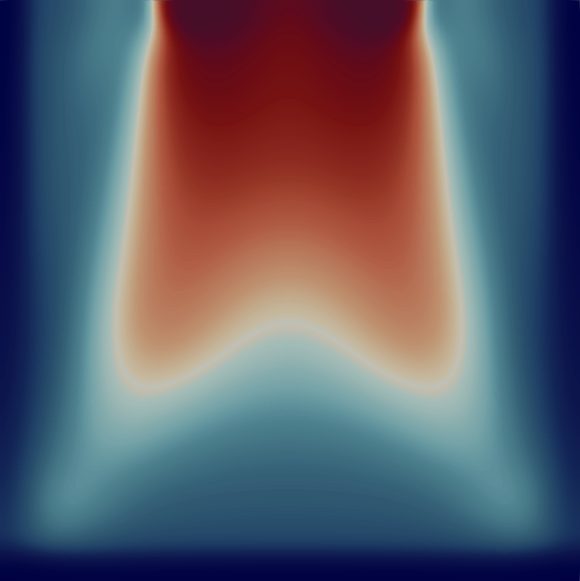
\includegraphics[width=\textwidth]{imgs/UnitSquare_1/second.png}
        \caption{$t = 6$}
    \end{subfigure}
    \begin{subfigure}{.4\textwidth}
        
\includegraphics[width=\textwidth]{imgs/UnitSquare_1/third.png}
        \caption{$t = 13$}
    \end{subfigure}
    \begin{subfigure}{.4\textwidth}
        
\includegraphics[width=\textwidth]{imgs/UnitSquare_1/fourth.png}
        \caption{$t = 20$}
    \end{subfigure}
    \begin{subfigure}{.4\textwidth}
        
\includegraphics[width=\textwidth]{imgs/UnitSquare_1/fifth.png}
        \caption{$t = 27$}
    \end{subfigure}
    \begin{subfigure}{.4\textwidth}
        
\includegraphics[width=\textwidth]{imgs/UnitSquare_1/sixth.png}
        \caption{$t = 35$}
    \end{subfigure}
    \begin{subfigure}{.4\textwidth}
        
\includegraphics[width=\textwidth]{imgs/UnitSquare_1/seventh.png}
        \caption{$t = 51$}
    \end{subfigure}
    \begin{subfigure}{.4\textwidth}
        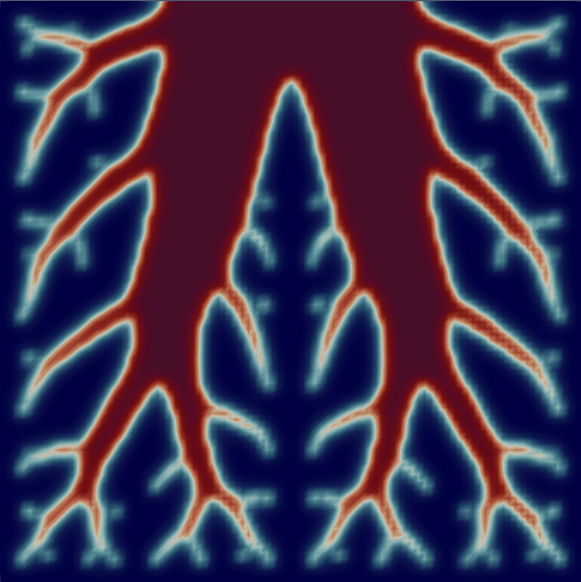
\includegraphics[width=\textwidth]{imgs/UnitSquare_1/eighth.png}
        \caption{$t = 65$}
    \end{subfigure}
\end{figure}

\vfill\pagebreak

\begin{figure}[H]
    \centering
    \caption{Unit Square with Single Sink: State Solution}
    \begin{subfigure}{.4\textwidth}
        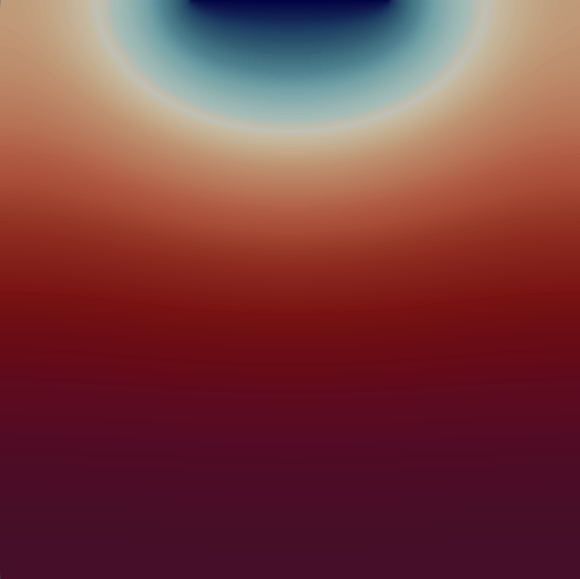
\includegraphics[width=\textwidth]{imgs/UnitSquare1_State/first.png}
        \caption{$t = 1$}
    \end{subfigure}
    \begin{subfigure}{.4\textwidth}
        
\includegraphics[width=\textwidth]{imgs/UnitSquare1_State/second.png}
        \caption{$t = 6$}
    \end{subfigure}
    \begin{subfigure}{.4\textwidth}
        
\includegraphics[width=\textwidth]{imgs/UnitSquare1_State/third.png}
        \caption{$t = 13$}
    \end{subfigure}
    \begin{subfigure}{.4\textwidth}
        
\includegraphics[width=\textwidth]{imgs/UnitSquare1_State/fourth.png}
        \caption{$t = 20$}
    \end{subfigure}
    \begin{subfigure}{.4\textwidth}
        
\includegraphics[width=\textwidth]{imgs/UnitSquare1_State/fifth.png}
        \caption{$t = 27$}
    \end{subfigure}
    \begin{subfigure}{.4\textwidth}
        
\includegraphics[width=\textwidth]{imgs/UnitSquare1_State/sixth.png}
        \caption{$t = 35$}
    \end{subfigure}
    \begin{subfigure}{.4\textwidth}
        
\includegraphics[width=\textwidth]{imgs/UnitSquare1_State/seventh.png}
        \caption{$t = 51$}
    \end{subfigure}
    \begin{subfigure}{.4\textwidth}
        
\includegraphics[width=\textwidth]{imgs/UnitSquare1_State/eighth.png}
        \caption{$t = 65$}
    \end{subfigure}
\end{figure}

\vfill\pagebreak

\begin{figure}[H]
    \centering
    \caption{Unit Square with Two Sinks: Filtered Distribution}
    \begin{subfigure}{.4\textwidth}
        
\includegraphics[width=\textwidth]{imgs/UnitSquare2/first.png}
        \caption{$t = 2$}
    \end{subfigure}
    \begin{subfigure}{.4\textwidth}
        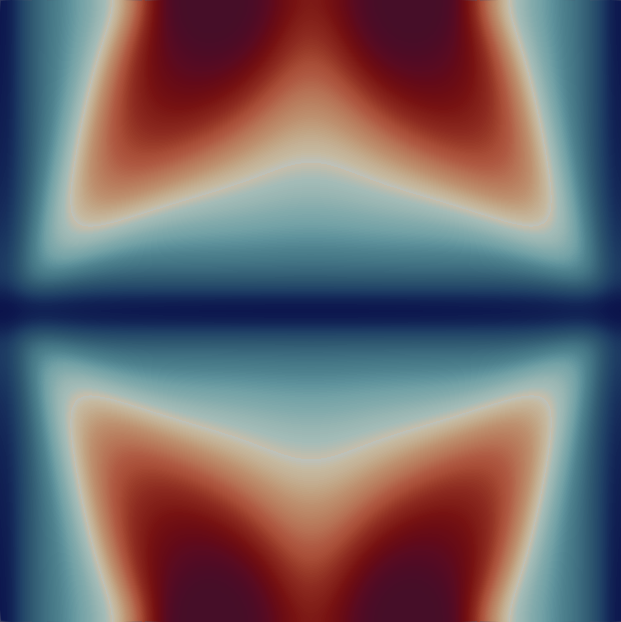
\includegraphics[width=\textwidth]{imgs/UnitSquare2/second.png}
        \caption{$t = 16$}
    \end{subfigure}
    \begin{subfigure}{.4\textwidth}
        
\includegraphics[width=\textwidth]{imgs/UnitSquare2/third.png}
        \caption{$t = 32$}
    \end{subfigure}
    \begin{subfigure}{.4\textwidth}
        
\includegraphics[width=\textwidth]{imgs/UnitSquare2/fourth.png}
        \caption{$t = 48$}
    \end{subfigure}
    \begin{subfigure}{.4\textwidth}
        
\includegraphics[width=\textwidth]{imgs/UnitSquare2/fifth.png}
        \caption{$t = 64$}
    \end{subfigure}
    \begin{subfigure}{.4\textwidth}
        
\includegraphics[width=\textwidth]{imgs/UnitSquare2/sixth.png}
        \caption{$t = 80$}
    \end{subfigure}
    \begin{subfigure}{.4\textwidth}
        
\includegraphics[width=\textwidth]{imgs/UnitSquare2/seventh.png}
        \caption{$t = 96$}
    \end{subfigure}
    \begin{subfigure}{.4\textwidth}
        
\includegraphics[width=\textwidth]{imgs/UnitSquare2/eighth.png}
        \caption{$t = 127$}
    \end{subfigure}
\end{figure}

\vfill\pagebreak

\begin{figure}[H]
    \centering
    \caption{Unit Square with Two Sinks Simulation: State Solution}
    \begin{subfigure}{.4\textwidth}
        
\includegraphics[width=\textwidth]{imgs/UnitSquare2_State/first.png}
        \caption{$t = 2$}
    \end{subfigure}
    \begin{subfigure}{.4\textwidth}
        
\includegraphics[width=\textwidth]{imgs/UnitSquare2_State/second.png}
        \caption{$t = 16$}
    \end{subfigure}
    \begin{subfigure}{.4\textwidth}
        
\includegraphics[width=\textwidth]{imgs/UnitSquare2_State/third.png}
        \caption{$t = 32$}
    \end{subfigure}
    \begin{subfigure}{.4\textwidth}
        
\includegraphics[width=\textwidth]{imgs/UnitSquare2_State/fourth.png}
        \caption{$t = 48$}
    \end{subfigure}
    \begin{subfigure}{.4\textwidth}
        
\includegraphics[width=\textwidth]{imgs/UnitSquare2_State/fifth.png}
        \caption{$t = 64$}
    \end{subfigure}
    \begin{subfigure}{.4\textwidth}
        
\includegraphics[width=\textwidth]{imgs/UnitSquare2_State/sixth.png}
        \caption{$t = 80$}
    \end{subfigure}
    \begin{subfigure}{.4\textwidth}
        
\includegraphics[width=\textwidth]{imgs/UnitSquare2_State/seventh.png}
        \caption{$t = 96$}
    \end{subfigure}
    \begin{subfigure}{.4\textwidth}
        
\includegraphics[width=\textwidth]{imgs/UnitSquare2_State/eighth.png}
        \caption{$t = 127$}
    \end{subfigure}
\end{figure}

\vfill\pagebreak

\subsubsection{$L$-shaped Domain with a Single Sink}

Here, now over an $L$-shaped domain, we allow for heat to escape part of the top edge. The interior is
also constantly and uniformly heated. The problem remains otherwise the same.

\begin{figure}[H]
    \centering
    \caption[b]{$L$-shaped $\Omega$ with a sink.}
    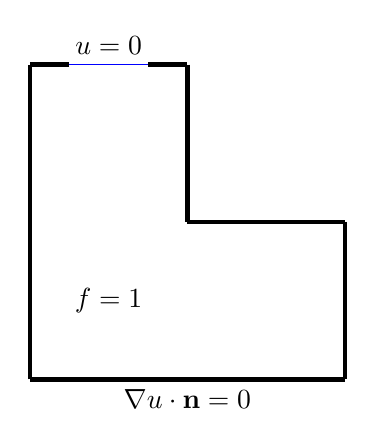
\begin{tikzpicture}
        \draw [ultra thick] (0,0) -- (4,0);
        \draw [ultra thick] (0,0) -- (0,4);

        \draw [ultra thick] (0,4) -- (0.5,4);
        \draw [blue] (0.5,4) -- (1.5,4);
        \draw [ultra thick] (1.5,4) -- (2,4);

        \draw [ultra thick] (2,4) -- (2,2);
        \draw [ultra thick] (2,2) -- (4,2);
        \draw [ultra thick] (4,2) -- (4,0);
        

        \node at (1, 4) [anchor = south] {$u = 0$};
        \node at (1, 1) {$f = 1$};
        \node at (2, 0) [anchor = north] {$\nabla u \cdot \mathbf{n} = 0$};
    \end{tikzpicture}
\end{figure}

We again see the tree-like structure here, maximizing surface area; intuitively, that it wraps around the corner
is an artifact of the mass constraint and that it needs to reach the south-east corner. The simulation was run
with $\theta = 0.5$ and $\alpha = 0.001$.

\subsubsection{$L$-shaped Domain with a Sink and a Source}

We will again allow for heat to escape part of the top edge, but instead of constant heating throughout, we will
consider only a source (marked in red; corresponding to given non-homogeneous Neumann boundary conditions) on the right edge.

\begin{figure}[H]
    \centering
    \caption[b]{$L$-shaped $\Omega$ with a sink and source.}
    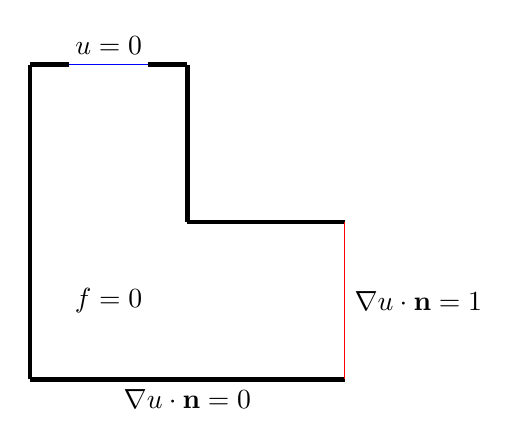
\begin{tikzpicture}
        \draw [ultra thick] (0,0) -- (4,0);
        \draw [ultra thick] (0,0) -- (0,4);

        \draw [ultra thick] (0,4) -- (0.5,4);
        \draw [blue] (0.5,4) -- (1.5,4);
        \draw [ultra thick] (1.5,4) -- (2,4);

        \draw [ultra thick] (2,4) -- (2,2);
        \draw [ultra thick] (2,2) -- (4,2);
        \draw [red] (4,2) -- (4,0);
        

        \node at (1, 4) [anchor = south] {$u = 0$};
        \node at (1, 1) {$f = 0$};
        \node at (4, 1) [anchor = west] {$\nabla u \cdot \mathbf{n} = 1$};
        \node at (2, 0) [anchor = north] {$\nabla u \cdot \mathbf{n} = 0$};
    \end{tikzpicture}
\end{figure}

On the physicality of this solution, we can interpret this as simply taking the shortest path to distribute
the heat to the sink. This simulation was also run with $\theta = 0.5$ and $\alpha = 0.001$.

\vfill\pagebreak

\begin{figure}[H]
    \centering
    \caption{$L$-shape with a Sink: Filtered Distribution}
    \begin{subfigure}{.4\textwidth}
        
\includegraphics[width=\textwidth]{imgs/LShape/first.png}
        \caption{$t = 2$}
    \end{subfigure}
    \begin{subfigure}{.4\textwidth}
        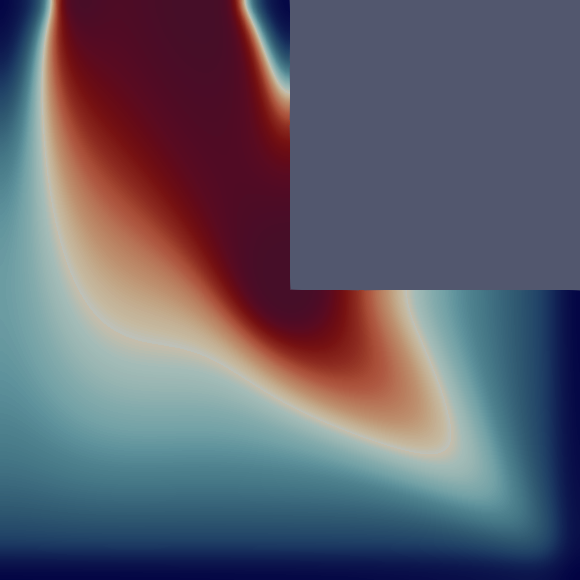
\includegraphics[width=\textwidth]{imgs/LShape/second.png}
        \caption{$t = 25$}
    \end{subfigure}
    \begin{subfigure}{.4\textwidth}
        
\includegraphics[width=\textwidth]{imgs/LShape/third.png}
        \caption{$t = 50$}
    \end{subfigure}
    \begin{subfigure}{.4\textwidth}
        
\includegraphics[width=\textwidth]{imgs/LShape/fourth.png}
        \caption{$t = 75$}
    \end{subfigure}
    \begin{subfigure}{.4\textwidth}
        
\includegraphics[width=\textwidth]{imgs/LShape/fifth.png}
        \caption{$t = 100$}
    \end{subfigure}
    \begin{subfigure}{.4\textwidth}
        
\includegraphics[width=\textwidth]{imgs/LShape/sixth.png}
        \caption{$t = 125$}
    \end{subfigure}
    \begin{subfigure}{.4\textwidth}
        
\includegraphics[width=\textwidth]{imgs/LShape/seventh.png}
        \caption{$t = 175$}
    \end{subfigure}
    \begin{subfigure}{.4\textwidth}
        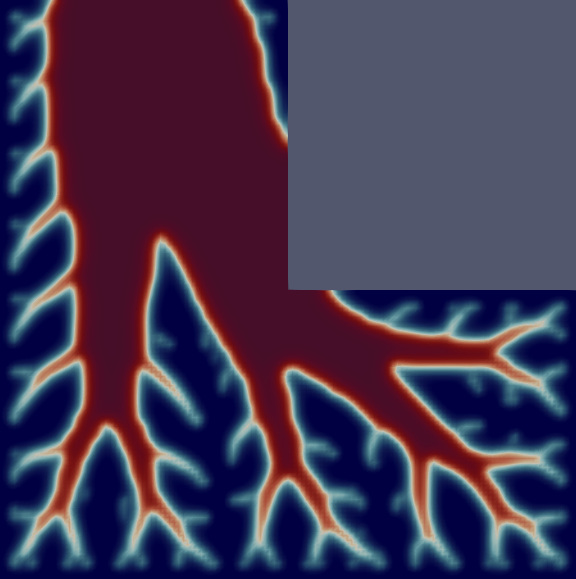
\includegraphics[width=\textwidth]{imgs/LShape/eighth.png}
        \caption{$t = 225$}
    \end{subfigure}
\end{figure}

\vfill\pagebreak

\begin{figure}[H]
    \centering
    \caption{$L$-shape with a Sink: State Solution}
    \begin{subfigure}{.4\textwidth}
        
\includegraphics[width=\textwidth]{imgs/LShape_Solution/first.png}
        \caption{$t = 2$}
    \end{subfigure}
    \begin{subfigure}{.4\textwidth}
        
\includegraphics[width=\textwidth]{imgs/LShape_Solution/second.png}
        \caption{$t = 25$}
    \end{subfigure}
    \begin{subfigure}{.4\textwidth}
        
\includegraphics[width=\textwidth]{imgs/LShape_Solution/third.png}
        \caption{$t = 50$}
    \end{subfigure}
    \begin{subfigure}{.4\textwidth}
        
\includegraphics[width=\textwidth]{imgs/LShape_Solution/fourth.png}
        \caption{$t = 75$}
    \end{subfigure}
    \begin{subfigure}{.4\textwidth}
        
\includegraphics[width=\textwidth]{imgs/LShape_Solution/fifth.png}
        \caption{$t = 100$}
    \end{subfigure}
    \begin{subfigure}{.4\textwidth}
        
\includegraphics[width=\textwidth]{imgs/LShape_Solution/sixth.png}
        \caption{$t = 125$}
    \end{subfigure}
    \begin{subfigure}{.4\textwidth}
        
\includegraphics[width=\textwidth]{imgs/LShape_Solution/seventh.png}
        \caption{$t = 175$}
    \end{subfigure}
    \begin{subfigure}{.4\textwidth}
        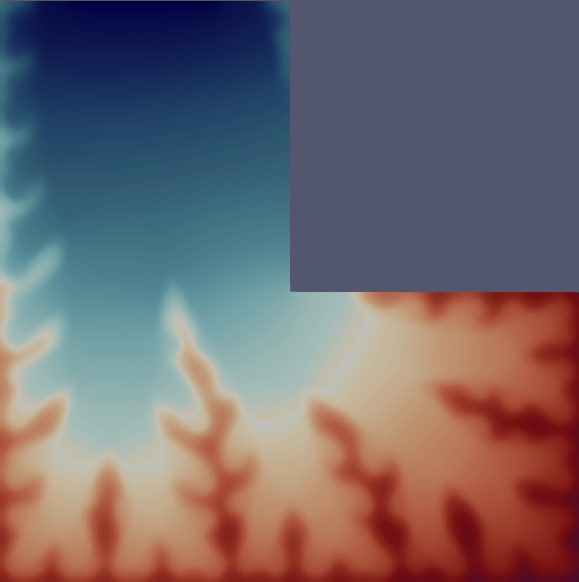
\includegraphics[width=\textwidth]{imgs/LShape_Solution/eighth.png}
        \caption{$t = 225$}
    \end{subfigure}
\end{figure}


\vfill\pagebreak

\begin{figure}[H]
    \centering
    \caption{$L$-shape with a Sink and Source: Filtered Distribution}
    \begin{subfigure}{.4\textwidth}
        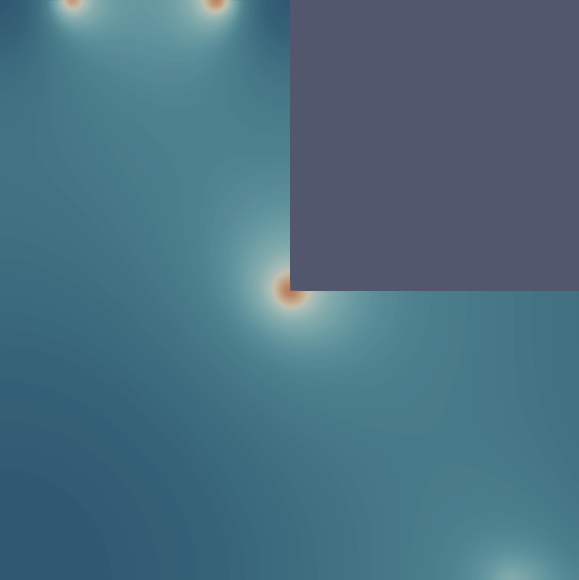
\includegraphics[width=\textwidth]{imgs/LShapeSource/first.png}
        \caption{$t = 3$}
    \end{subfigure}
    \begin{subfigure}{.4\textwidth}
        
\includegraphics[width=\textwidth]{imgs/LShapeSource/second.png}
        \caption{$t = 8$}
    \end{subfigure}
    \begin{subfigure}{.4\textwidth}
        \includegraphics[width=\textwidth]{imgs/LShapeSource/third.png}
        \caption{$t = 12$}
    \end{subfigure}
    \begin{subfigure}{.4\textwidth}
        \includegraphics[width=\textwidth]{imgs/LShapeSource/fourth.png}
        \caption{$t = 18$}
    \end{subfigure}
    \begin{subfigure}{.4\textwidth}
        \includegraphics[width=\textwidth]{imgs/LShapeSource/fifth.png}
        \caption{$t = 26$}
    \end{subfigure}
    \begin{subfigure}{.4\textwidth}
        \includegraphics[width=\textwidth]{imgs/LShapeSource/sixth.png}
        \caption{$t = 34$}
    \end{subfigure}
    \begin{subfigure}{.4\textwidth}
        \includegraphics[width=\textwidth]{imgs/LShapeSource/seventh.png}
        \caption{$t = 45$}
    \end{subfigure}
    \begin{subfigure}{.4\textwidth}
        \includegraphics[width=\textwidth]{imgs/LShapeSource/eighth.png}
        \caption{$t = 80$}
    \end{subfigure}
\end{figure}

\vfill\pagebreak

\begin{figure}[H]
    \centering
    \caption{$L$-shape with a Sink and Source: State Solution}
    \begin{subfigure}{.4\textwidth}
        \includegraphics[width=\textwidth]{imgs/LShapeSource_Solution/first.png}
        \caption{$t = 3$}
    \end{subfigure}
    \begin{subfigure}{.4\textwidth}
        \includegraphics[width=\textwidth]{imgs/LShapeSource_Solution/second.png}
        \caption{$t = 8$}
    \end{subfigure}
    \begin{subfigure}{.4\textwidth}
        \includegraphics[width=\textwidth]{imgs/LShapeSource_Solution/third.png}
        \caption{$t = 12$}
    \end{subfigure}
    \begin{subfigure}{.4\textwidth}
        \includegraphics[width=\textwidth]{imgs/LShapeSource_Solution/fourth.png}
        \caption{$t = 18$}
    \end{subfigure}
    \begin{subfigure}{.4\textwidth}
        \includegraphics[width=\textwidth]{imgs/LShapeSource_Solution/fifth.png}
        \caption{$t = 26$}
    \end{subfigure}
    \begin{subfigure}{.4\textwidth}
        \includegraphics[width=\textwidth]{imgs/LShapeSource_Solution/sixth.png}
        \caption{$t = 34$}
    \end{subfigure}
    \begin{subfigure}{.4\textwidth}
        \includegraphics[width=\textwidth]{imgs/LShapeSource_Solution/seventh.png}
        \caption{$t = 45$}
    \end{subfigure}
    \begin{subfigure}{.4\textwidth}
        \includegraphics[width=\textwidth]{imgs/LShapeSource_Solution/eighth.png}
        \caption{$t = 80$}
    \end{subfigure}
\end{figure}

\vfill\pagebreak

\subsubsection{CPU Heat Sink Problem}

Finally, we will consider a heat sink design problem, where the heat source is embedded within our design space $\Omega$;
on the ``internal boundary'' formed by the presence of this source, eg, a computer processor, we will impose nonhomogeneous Neumann BCs.
Heat is allowed to escape on the left and right edges, where we might imagine there is a connection to a larger
heatsink.

\begin{figure}[H]
    \centering
    \caption[b]{Heat-sink problem.}
    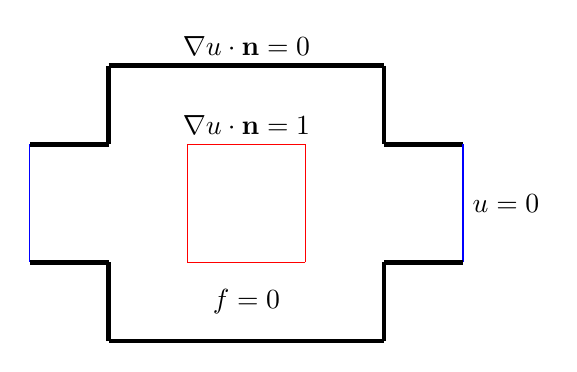
\begin{tikzpicture}
        \draw [red] (0,0) -- (1.5,0);
        \draw [red] (0,0) -- (0,1.5);
        \draw [red] (1.5,0) -- (1.5,1.5);
        \draw [red] (0,1.5) -- (1.5,1.5);

        \draw [ultra thick] (-1,-1) -- (2.5,-1);
        \draw [ultra thick] (-1,2.5) -- (2.5,2.5);
        \draw [ultra thick] (-1,-1) -- (-1,0);
        \draw [ultra thick] (2.5,-1) -- (2.5,0);
        \draw [ultra thick] (-1,2.5) -- (-1,1.5);
        \draw [ultra thick] (2.5,2.5) -- (2.5,1.5);

        \draw [ultra thick] (2.5,1.5) -- (3.5,1.5);
        \draw [blue] (3.5,1.5) -- (3.5,0);
        \draw [ultra thick] (3.5,0) -- (2.5,0);

        \draw [ultra thick] (-1,1.5) -- (-2,1.5);
        \draw [blue] (-2,1.5) -- (-2,0);
        \draw [ultra thick] (-1,0) -- (-2,0);

        \node at (3.5, 0.75) [anchor = west] {$u = 0$};
        \node at (0.75, -0.5) {$f = 0$};
        \node at (0.75, 1.5) [anchor = south] {$\nabla u \cdot \mathbf{n} = 1$};
        \node at (0.75,2.5) [anchor = south] {$\nabla u \cdot \mathbf{n} = 0$};

    \end{tikzpicture}
\end{figure}


\vfill\pagebreak

\begin{figure}[H]
    \centering
    \caption{Heat sink problem: Filtered Distribution}
    \begin{subfigure}{.4\textwidth}
        \includegraphics[width=\textwidth]{imgs/HeatSink/first.png}
        \caption{$t = 2$}
    \end{subfigure}
    \begin{subfigure}{.4\textwidth}
        \includegraphics[width=\textwidth]{imgs/HeatSink/second.png}
        \caption{$t = 5$}
    \end{subfigure}
    \begin{subfigure}{.4\textwidth}
        \includegraphics[width=\textwidth]{imgs/HeatSink/third.png}
        \caption{$t = 8$}
    \end{subfigure}
    \begin{subfigure}{.4\textwidth}
        \includegraphics[width=\textwidth]{imgs/HeatSink/fourth.png}
        \caption{$t = 30$}
    \end{subfigure}
    \begin{subfigure}{.4\textwidth}
        \includegraphics[width=\textwidth]{imgs/HeatSink/fifth.png}
        \caption{$t = 60$}
    \end{subfigure}
    \begin{subfigure}{.4\textwidth}
        \includegraphics[width=\textwidth]{imgs/HeatSink/sixth.png}
        \caption{$t = 90$}
    \end{subfigure}
    \begin{subfigure}{.4\textwidth}
        \includegraphics[width=\textwidth]{imgs/HeatSink/seventh.png}
        \caption{$t = 120$}
    \end{subfigure}
    \begin{subfigure}{.4\textwidth}
        \includegraphics[width=\textwidth]{imgs/HeatSink/eighth.png}
        \caption{$t = 150$}
    \end{subfigure}
\end{figure}

\vfill\pagebreak

\begin{figure}[H]
    \centering
    \caption{Heat sink problem: State Solution}
    \begin{subfigure}{.4\textwidth}
        \includegraphics[width=\textwidth]{imgs/HeatSink_Solution/first.png}
        \caption{$t = 2$}
    \end{subfigure}
    \begin{subfigure}{.4\textwidth}
        \includegraphics[width=\textwidth]{imgs/HeatSink_Solution/second.png}
        \caption{$t = 5$}
    \end{subfigure}
    \begin{subfigure}{.4\textwidth}
        \includegraphics[width=\textwidth]{imgs/HeatSink_Solution/third.png}
        \caption{$t = 8$}
    \end{subfigure}
    \begin{subfigure}{.4\textwidth}
        \includegraphics[width=\textwidth]{imgs/HeatSink_Solution/fourth.png}
        \caption{$t = 30$}
    \end{subfigure}
    \begin{subfigure}{.4\textwidth}
        \includegraphics[width=\textwidth]{imgs/HeatSink_Solution/fifth.png}
        \caption{$t = 60$}
    \end{subfigure}
    \begin{subfigure}{.4\textwidth}
        \includegraphics[width=\textwidth]{imgs/HeatSink_Solution/sixth.png}
        \caption{$t = 90$}
    \end{subfigure}
    \begin{subfigure}{.4\textwidth}
        \includegraphics[width=\textwidth]{imgs/HeatSink_Solution/seventh.png}
        \caption{$t = 120$}
    \end{subfigure}
    \begin{subfigure}{.4\textwidth}
        \includegraphics[width=\textwidth]{imgs/HeatSink_Solution/eighth.png}
        \caption{$t = 150$}
    \end{subfigure}
\end{figure}

\vfill\pagebreak

